\subsection{Desenvolvimento}

\par A princípio, utilizou-se as tecnologias Neo4j, sendo executado de forma \textit{embedded}, Primefaces e JSF. Porém não estava fluindo como o esperado. Outro problema encontrado ao utilizar tais tecnologias foi que tanto a parte cliente (\textit{front end}) quanto a parte servidor (\textit{back end}) se encontravam totalmente acoplados em uma aplicação Java \textit{web}. Por estes motivos decidiu-se mudar algumas das tecnologias utilizadas.

\par Posterior a esse incidente, passou-se a utilizar então as linguagens HTML 5, CSS 3, Javascript e o \textit{framework} Angular JS para auxiliar no desenvolvimento do \textit{front end}, ao invés de Primefaces e JSF. Para acesso ao banco de dados, lançou-se mão da forma \textit{embedded} e passou-se a utilizar a API REST disponibilizada pelo próprio banco. Tais decisões nos permitiram desacoplar o sistema e manter o \textit{front end} e o \textit{back end} independentes, evitando, assim, que o mesmo problema voltasse a ocorrer.

\par Como a forma de conexão ao banco de dados foi alterada, houve a necessidade de reescrever a classe responsável por realizar esta conexão, conforme apresenta o Código~\ref{list:codigo_comunicacao_banco}.

\begin{lstlisting} [style=custom_Java,caption={[Código de comunicação com o banco de dados]{Código de comunicação com o banco de dados. \textbf{Fonte:} Elaborado pelos autores.}}, label=list:codigo_comunicacao_banco]
public class FactoryDAO {

	private static final String DATABASE_ENDPOINT =
								 "http://localhost:7474/db/data";
	private static final String DATABASE_USERNAME = "neo4j";
	private static final String DATABASE_PASSWORD = "admin";
	private static final String cypherUrl = 
								 DATABASE_ENDPOINT + "/cypher";
	
	private static WebResource instance;
	
	private FactoryDAO() {
	}
	
	public static WebResource GetInstance() {
		WebResource resource = null;
		if (instance == null) {
			Client c = Client.create();
			c.addFilter(new HTTPBasicAuthFilter(DATABASE_USERNAME,
												DATABASE_PASSWORD));
			resource = c.resource(cypherUrl);
		}
		return resource;
	}
}
\end{lstlisting}

% Trocado de imagem para listagem
%\begin{figure}[h!]
%	\centerline{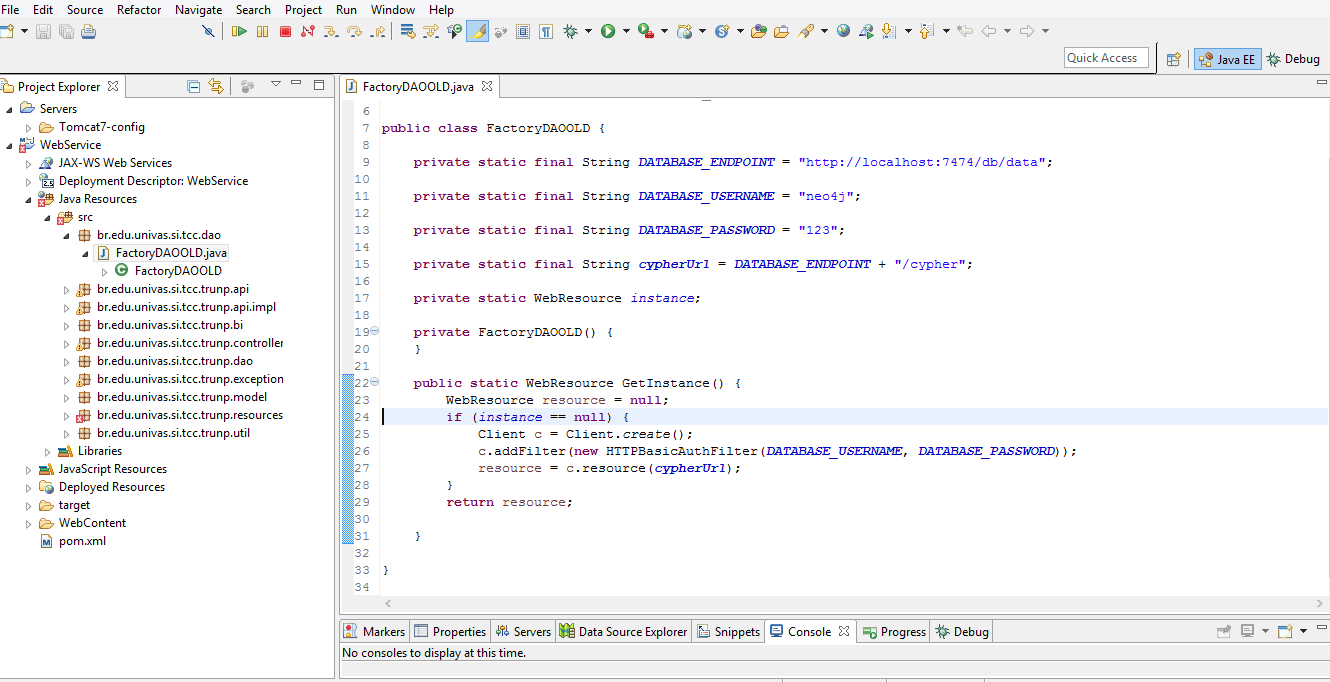
\includegraphics[scale=0.3]{./imagens/conexao-banco.jpg}}
%	\caption[Código de comunicação com o banco]
%	{Código de comunicação com o banco \textbf{Fonte:} Elaborado pelos autores.}
%	\label{fig:codigo_comunicacao_banco}
%\end{figure}

\par Após realizar a mudança de tecnologias, foram executados alguns procedimentos para compreender o funcionamento do \textit{web service} REST e em paralelo, foi feito o levantamento dos materiais de referência do \textit{framework} Angular JS. Foi preciso realizar testes para validar a conexão com o banco de dados Neo4j via API REST, fornecida por ele, além de realizados testes funcionais para envio de requisições e recebimento de respostas do \textit{web service} REST, utilizando o Angular JS. Para validar a conexão ao banco de dados via API REST foi necessário desenvolver algumas consultas em \textit{cypher}, como apresenta o Código~\ref{list:consulta_usando_api_cypher}.

\begin{lstlisting} [style=custom_Java,caption={[Exemplo de consulta usando a API \textit{cypher}]{Exemplo de consulta usando a API \textit{cypher}. \textbf{Fonte:} Elaborado pelos autores.}}, label=list:consulta_usando_api_cypher] 	

public class PersonDAO {
...

	/**
	* Used to get all data of person to show the profile data
	* 
	* @param partnerEmail
	* @return
	* @throws JSONException 
	*/
	public JSONArray getPersonData(String partnerEmail) throws JSONException {
		
		WebResource resource = FactoryDAO.GetInstance();
		
		String query = null;
		query = "{\"query\":\" MATCH (partner:Person {email: '"
			+ partnerEmail + "'}), (city:City), "
			+ "(company:Company), "
			+ "(partner)-[:LIVES_IN]->(city), "
			+ "(partner)-[:WORKS_IN]->(company) "
			+ "RETURN DISTINCT({name: partner.name, "
			+ "email: partner.email, photo: partner.photo, " 
			+ "city: city.name, company: company.name, " 
			+ "cpf: partner.cpf, cnpj: partner.cnpj, " 
			+ "typeOfPerson: partner.typeOfPerson, " 
			+ "gender: partner.gender}) as partner; \"}";
		ClientResponse responseCreate = resource
									.accept(MediaType.APPLICATION_JSON)
									.type(MediaType.APPLICATION_JSON).entity(query)
									.post(ClientResponse.class);
		String resp = responseCreate.getEntity(String.class);
		
		JSONObject json = new JSONObject(resp);
		JSONArray objData = json.getJSONArray("data");
		List<JSONObject> parser = JSONUtil
												.parseJSONArrayToListJSON(objData);
		JSONArray arr = new JSONArray(parser);
		
		return arr;
	}
...
}
\end{lstlisting}

% Trocado de imagem para listagem
%\begin{figure}[h!]
%	\centerline{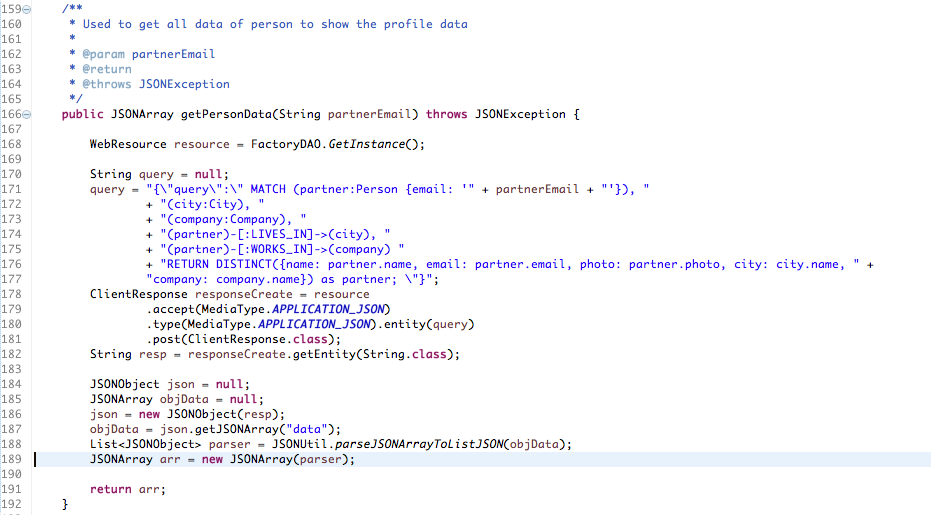
\includegraphics[scale=0.45]{./imagens/query-cypher.png}}
%	\caption[Exemplo de consulta usando a API \textit{cypher}]
%	{Exemplo de consulta usando a API \textit{cypher}. \textbf{Fonte:} Elaborado pelos autores.}
%	\label{fig:consulta_usando_api_cypher}
%\end{figure}

Nesse trecho de código entre as linhas 17 e 27 é apresentada uma consulta escrita usando a API \textit{Cypher}, ela tem por finalidade recuperar os dados de um determinado usuário. Como já mencionado no quadro teórico deste trabalho, o \textit{Cypher} utiliza algumas cláusulas, dentre elas é possível mencionar a \texttt{MATCH} e \texttt{RETURN} cuja utilização delas é apresentada nessa consulta. Na cláusula \texttt{MATCH} são definidos os padrões para realizar a busca, nesse caso, uma pessoa que viva em qualquer cidade, trabalhe em uma empresa qualquer e que possua o \textit{e-mail} igual ao recebido como parâmetro pelo método \texttt{getPersonData}. Já a clásula \texttt{RETURN}, são definidos os dados desejados pela consulta, nesse caso, são eles: o nome do usuário, o \textit{e-mail}, a foto, a cidade onde vive, a empresa onde trabalha, o CPF (em caso de pessoas físicas), o CNPJ (para pessoas jurídicas), o tipo da conta (pessoa jurídica ou física), e o sexo do usuário (usado para pessoas físicas). Mas como é possível notar, foi necessário gerar um objeto JSON manualmente contendo os dados desejados como pode ser visualizado a partir da linha 22 até a linha 27, pois, por padrão o Neo4j não retorna os resultados no formato JSON comum, como demonstra o Código~\ref{list:exemplo_json_retornado_neo4j}. 

\begin{lstlisting} [style=custom_HTML,caption={[JSON retornado de uma consulta via \textit{Cypher}]{JSON retornado de uma consulta via \textit{Cypher}. \textbf{Fonte:} Elaborado pelos autores.}}, label=list:exemplo_json_retornado_neo4j] 	
{
	...
	column: [
		"name",
		"email",
		"password"
	],
	data: [
		"Andressa Faria",
		"andressa_faria18@hotmail.com",
		"78hweqroqy5brlfgvqpOIoi9uijkhgyteqwr"
	]
	...
}
\end{lstlisting}

Portanto, foi necessário desenvolver uma forma de converter os resultados obtidos nas buscas realizadas no banco de dados, a fim de retornar um JSON válido ao usuário, que futuramente viria a utilizar a API REST fornecida por este \textit{software}. É possível visualizar este tratamento no Código~\ref{list:consulta_usando_api_cypher} a partir da linha 34 até a linha 38.

Na linha 34 foi necessário criar um objeto JSON da classe \texttt{JSONObject} passando o retorno da consulta em seu construtor. Já na linha 35 foi obtido os dados retornados da consulta, porém, como demonstrado no Código~\ref{list:exemplo_json_retornado_neo4j} eles são retornados em uma \textit{collection} (coleção) e não em objetos, portanto, para obtê-los foi necessário criar um objeto da classe \texttt{JSONArray} e recuperá-los por meio do campo \texttt{data} do resultado.

Após recuperar os dados, foi necessário extraí-los dos resultados da consulta que até este ponto estavam armazenados em um \texttt{array} e transferí-los para uma lista de objetos da classe \texttt{JSONObject} como apresenta a linha 36 do Código~\ref{list:consulta_usando_api_cypher}, para tanto, foi criada uma classe estática denominada \texttt{JSONUtil} responsável por realizar essa tarefa e retonar os dados no formato padrão. Esse método é apresentado no Código~\ref{list:parser_jsonarray_to_list_json_object}.

\begin{lstlisting} [style=custom_JAVA,caption={[JSON padrão com os resultados das consultas \textit{Cypher}]{JSON padrão com os resultados das consultas \textit{Cypher}. \textbf{Fonte:} Elaborado pelos autores.}}, label=list:parser_jsonarray_to_list_json_object] 	
public class JSONUtil {
	...
	public static List<JSONObject>
									parseJSONArrayToListJSON(JSONArray array) throws JSONException {
		List<JSONObject> response = new ArrayList<JSONObject>();
		for (int i = 0; i < array.length(); i++) {
			JSONArray arr1 = array.getJSONArray(i);
			for (int j = 0; j < arr1.length(); j++) {
				JSONObject obj = arr1.getJSONObject(j);
				response.add(obj);
			}
		}
		return response;
	}
	...
}
\end{lstlisting}

Após essa extração de dados foi necessário criar um objeto da classe \texttt{JSONArray} passando o retorno do método \texttt{parseJSONArrayToListJSON} da classe \texttt{JSONUtil} em seu construtor, uma vez que, o limite de resultados obtidos em uma consulta depende, exclusivamente da própria consulta e da quantidade de registros armazenados no banco de dados. Após realizar todos esses passos, um objeto da classe \texttt{JSONArray} contendo todos os dados devidamente preenchidos é retornado para o método que requisitou essa consulta, como mostra a linha 38 e 40 do Código~\ref{list:consulta_usando_api_cypher}.
 
\par A partir deste ponto, a aplicação estava totalmente desacoplada, sendo necessário realizar uma configuração, a fim de permitir que as requisições enviadas pelo \textit{front end} fossem aceitas pelo \textit{back end}, localizado em outro domínio.

\par Devido à mudança de tecnologias já comentada, houve a necessidade de atualizar os diagramas de sequência e de classe, inserindo os contratos de serviços do \textit{web service} REST. Com a definição deste contrato que é apresentado no Apêndice II deste trabalho, deu-se início ao desenvolvimento dos casos de uso, identificados na primeira fase do ICONIX. 

\par Posterior à realização dos testes e da escolha definitiva da arquitetura que seria utilizada, iniciou-se a implementação dos casos de uso. O primeiro a ser implementado foi o caso de uso de criação de conta. Para este caso de uso, teve-se o cuidado de criar um mecanismo de criptografia de dados sigilosos, como usuário e senha, visando garantir a segurança da aplicação. Estas informações criptografadas são enviadas a cada requisição e validadas pelo \textit{web service}, sendo atualizadas caso sejam válidas, tornado mais complexo a quebra desta criptografia. Este mecanismo foi desenvolvido com base no sistema de \textit{login} via \textit{token}. Segundo o embasamento usado na criação de contas, deu-se início ao desenvolvimento do sistema de \textit{login} e \textit{logoff}, que também utilizam o conceito de criptografia via \textit{token}. A Figura~\ref{fig:pagina_login} apresenta a página de \textit{login}.

\begin{figure}[h!]
	\centerline{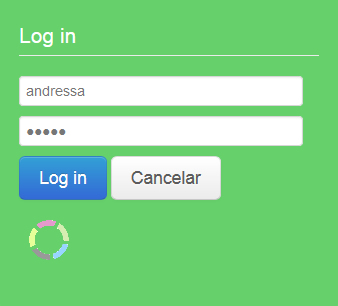
\includegraphics[scale=0.60]{./imagens/login.jpg}}
	\caption[Tela de \textit{log in}.]
	{Tela de \textit{log in}. \textbf{Fonte:} Elaborado pelos autores.}
	\label{fig:pagina_login}
\end{figure}

Segundo \citeonline{token_traditional_babal}, os sistemas de autenticações tradicionais utilizam recursos como sessão e \textit{cookies}. A autenticação do usuário é realizada por meio de alguns dados, geralmente nome de usuário (ou email) e senha, com esses dados a aplicação no \textit{back-end}, os validam junto a base de dados e caso obtenha sucesso nesse processo de validação é criada uma sessão e armazenada no servidor, após realizada toda a validação a aplicação retorna a informação dessa sessão para quem a requisitou de modo que ela seja armazenada no navegador de internet por meio de sessão e/ou \textit{cookies}. A partir desse momento, a cada nova solicitação a aplicação \textit{back-end} irá comparar a sessão armazenada no servidor com a fornecida pelo \textit{front-end}. A Figura~\ref{fig:autenticacao_via_sessao} demonstra o fluxo utilizado pelos sistemas cuja autenticação de sessão é a tradicional.

\begin{figure}[h!]
	\centerline{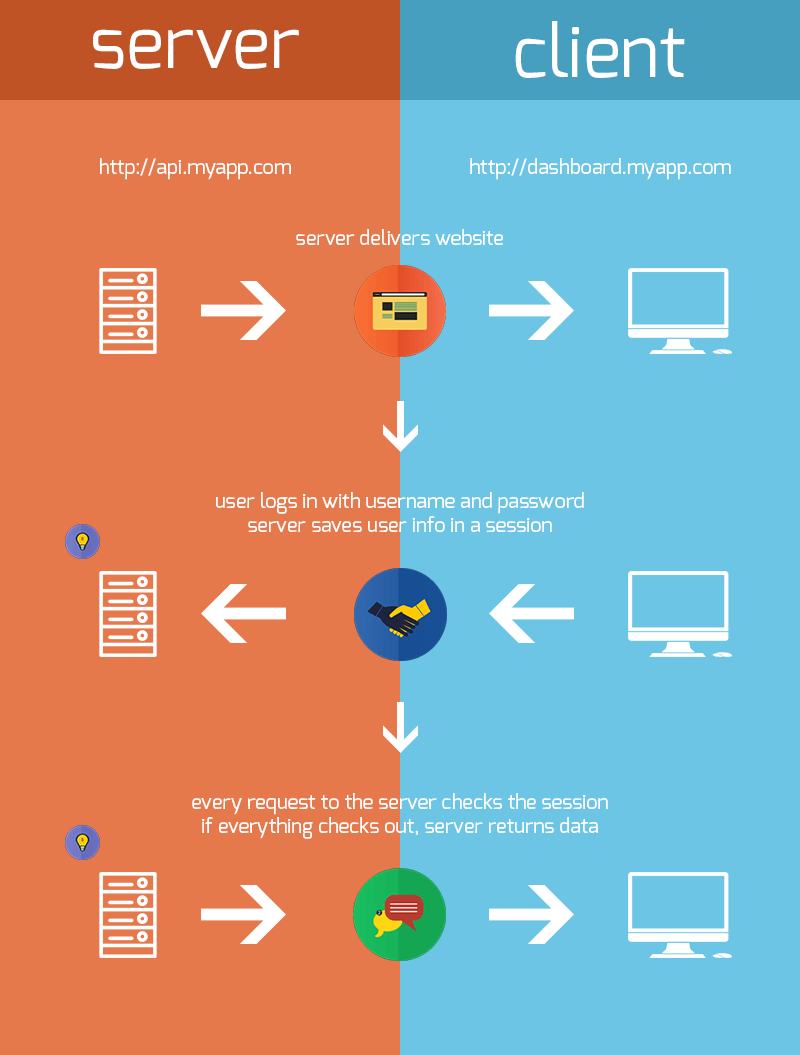
\includegraphics[scale=0.5]{./imagens/tokens-traditional.png}}
	\caption[Fluxo de autenticação de usuários utilizando a forma tradicional]
	{Fluxo de autenticação de usuários utilizando a forma tradicional. \textbf{Fonte:} \cite{authentication_via_token_chris_sevilleja}.}
	\label{fig:autenticacao_via_sessao}
\end{figure}

Para \citeonline{authentication_via_token_chris_sevilleja}, a autenticação via \textit{token}, diferente da forma convencional não utiliza os recursos de sessão e \textit{cookies}. Contudo o processo inicial é o mesmo, a autenticação se inicia por meio dos mesmos dados da forma tradicional, realizando o mesmo o processo de validação, junto à base de dados, porém caso obtenha sucesso não cria uma sessão, e sim um \textit{token} com os dados necessários para a sua validação \textit{criptografados}. Após criado o \textit{token} ele é enviado de volta ao usuário solicitante de modo que ele seja armazenado pela aplicação cliente, sendo ela um aplicativo \textit{web} ou \textit{mobile}, entre outras. A partir desse momento, a cada nova solicitação, a aplicação cliente deverá enviar o \textit{token} anteriormente recebido do servidor e armazenado por ela, para que ele seja validado. A Figura~\ref{fig:autenticacao_via_token} demonstra o fluxo utilizado pelos sistemas cuja autenticação é realizada via \textit{token}.

\newpage
\begin{figure}[h!]
	\centerline{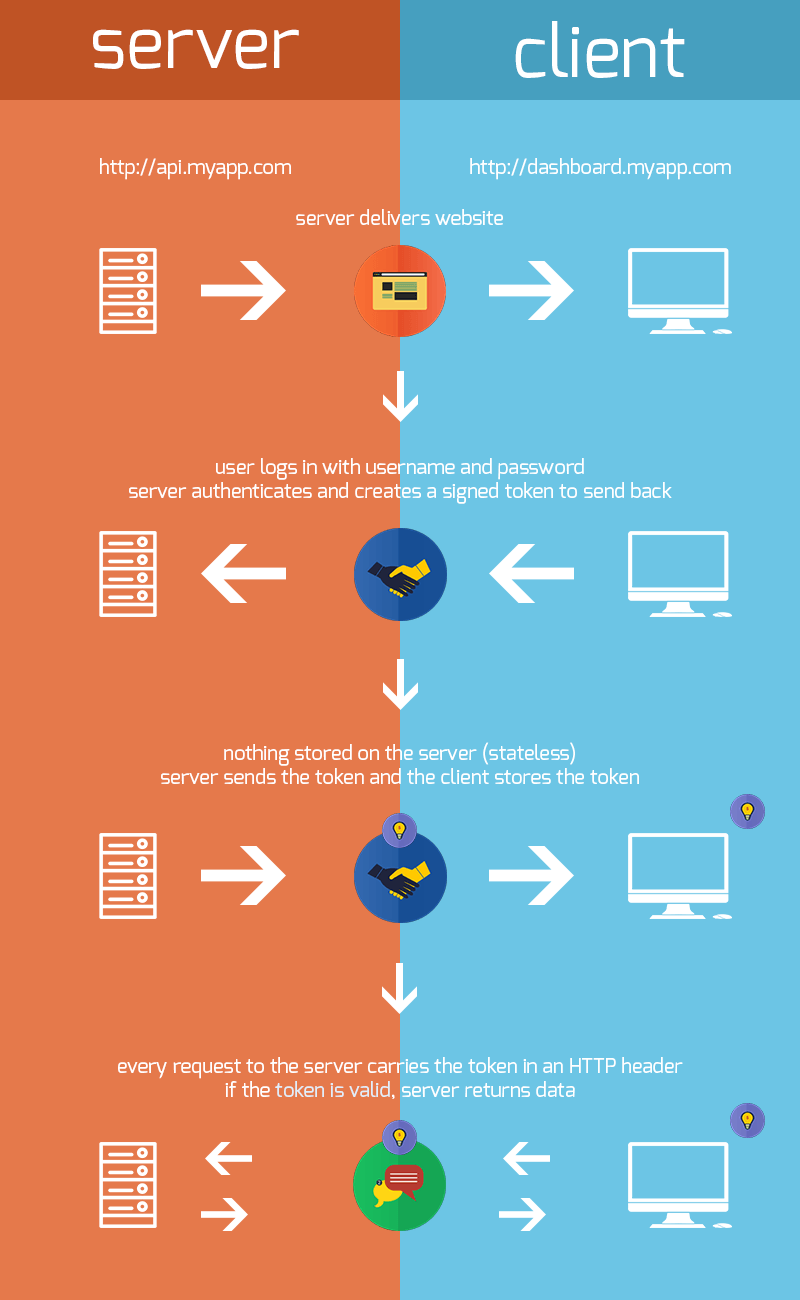
\includegraphics[scale=0.5]{./imagens/tokens-new.png}}
	\caption[Fluxo de autenticação de usuários utilizando \textit{token}]
	{Fluxo de autenticação de usuários utilizando \textit{token}. \textbf{Fonte:} \cite{authentication_via_token_chris_sevilleja}.}
	\label{fig:autenticacao_via_token}
\end{figure}

Para construir a aplicação seguindo o modelo de autenticação via \textit{token} foi necessário criar uma classe chamada \texttt{Base64Util} responsável por \textit{criptografar e descriptografar} as informações fornecidas no \textit{token} a fim de validá-lo junto a base de dados da aplicação. Essa classe é apresentada no Código~\ref{list:classe_criptografa_descriptografa_token}.

\begin{lstlisting} [style=custom_Java,caption={[Classe responsável pela criptografia e descriptografia do \textit{token}]{Classe responsável pela criptografia e descriptografia do \textit{token}. \textbf{Fonte:} Elaborado pelos autores.}}, label=list:classe_criptografa_descriptografa_token]
public class Base64Util {
	
	public static final String BASE64_TOKEN_SEPARATOR = "|";
	
	public static byte[] encodeToken(String email, String password) {
		/* Get Current Time in order to check if the session
		 * is valid yet.
		 */
		Long currentTime = new Timestamp(new Date().getTime()).getTime();
		byte[] token = Base64.encode(email + BASE64_TOKEN_SEPARATOR + password + BASE64_TOKEN_SEPARATOR + currentTime);
		return token;
	}
	
	public static Token decodeToken(byte[] tokenDecoded) {
		Token token = new Token();
		
		byte[] bytes = Base64.decode(tokenDecoded);
		String tokenStr = new String(bytes);
		
		String[] splitStr = tokenStr.split("\\" + BASE64_TOKEN_SEPARATOR);
		token.setEmail(splitStr[0]);
		token.setPassword(splitStr[1]);
		token.setLastAccessTime(Long.parseLong(splitStr[2]));
		
		return token;
	}
}
\end{lstlisting}

No código acima, o método chamado \texttt{encodeToken} recebe como parâmetro o \textit{e-mail} e a senha fornecidos pelo usuário no momento da realização do login, a partir dessas informações somado a hora atual do sistema que é obtida na linha 10 é gerado o \textit{token} criptografado em \texttt{Base64}. Para realizar a decodificação do \textit{token} é utilizado o método \texttt{decodeToken} cuja chamada é realizada a cada requisição que o cliente realiza, esse método recebe como parâmentro o \textit{token} criptografado e o descriptografa usando a classe \texttt{Base64} como é apresentado na linha 18. Após a descriptografia dele é criado um objeto da classe \texttt{Token} com as informações obtidas pelo \textit{token} fornecido pela requisição.

Diferentemente das aplicações que utilizam este conceito de sessão via \textit{token}, neste trabalho houve-se a necessidade de validar além das informações do usuário incluídas no próprio \textit{token}, a data e hora da última requisição realizada pelo usuário. Portanto, para validar o \textit{token} expirado foi necessário criar a classe \texttt{TokenBi} como demonstra o Código~\ref{list:classe_valida_token}.

\begin{lstlisting} [style=custom_Java,caption={[Classe responsável pela validação do \textit{token}]{Classe responsável pela validação do \textit{token}. \textbf{Fonte:} Elaborado pelos autores.}}, label=list:classe_valida_token]
public class TokenBi {
	
	private static final int MINUTES_OF_SESSION_ACTIVE = 15; //15min
	...
	
	/* Method to check if session is still alive */
	public boolean isExpiredSession(Token token) {
		
		final long ONE_MINUTE_IN_MILLIS = 60000;//millisecs
		
		Date currentTime = new Date();
		Date timeLastAccess = new Date(token.getLastAccessTime() 
				+ (MINUTES_OF_SESSION_ACTIVE * ONE_MINUTE_IN_MILLIS));
		
		if (timeLastAccess.before(currentTime)) {
			return true; //session already expired
		}
		return false; //session activate yet
	}
	...
}
\end{lstlisting}

Para realizar a validação do \textit{token} expirado, foi criado o método \texttt{isExpiredSession} que  recebe como parâmetro um objeto da classe \texttt{Token} contendo além dos dados do usuário, também a informação relacionada à data e hora da última requisição, com base nessa última informação na linha 12 é realizado um cálculo para obter um objeto do tipo \texttt{Date} contendo a data da última requisição do usuário somada a mais 15 minutos. A partir dessa informação é realizada uma comparação entre ela e a data atual do sistema, como é possível visualizar na linha 15, caso essa informação seja anterior a data atual do sistema o \textit{token} está expirado e o método \texttt{isExpiredSession} retorna \textit{true}. Caso contrário ele irá retornar \textit{false}.

\par Com o funcionamento do sistema de \textit{login}, passou-se a desenvolver a página inicial da aplicação, contendo as informações que são restritas ao usuário cadastrado. O sistema apresenta uma página inicial diferente para cada tipo de conta, sendo elas: contratantes, provedores de serviço ou ambos, contendo apenas as informações que são liberadas de acordo com o acesso do usuário, sendo essas relatórios, últimas atualizações na rede de parceiros, avaliações de serviços e prováveis parceiros. A página inicial do tipo contratante é apresentada na Figura~\ref{fig:pagina_inicial_contratante}.

\newpage
\begin{figure}[h!]
	\centerline{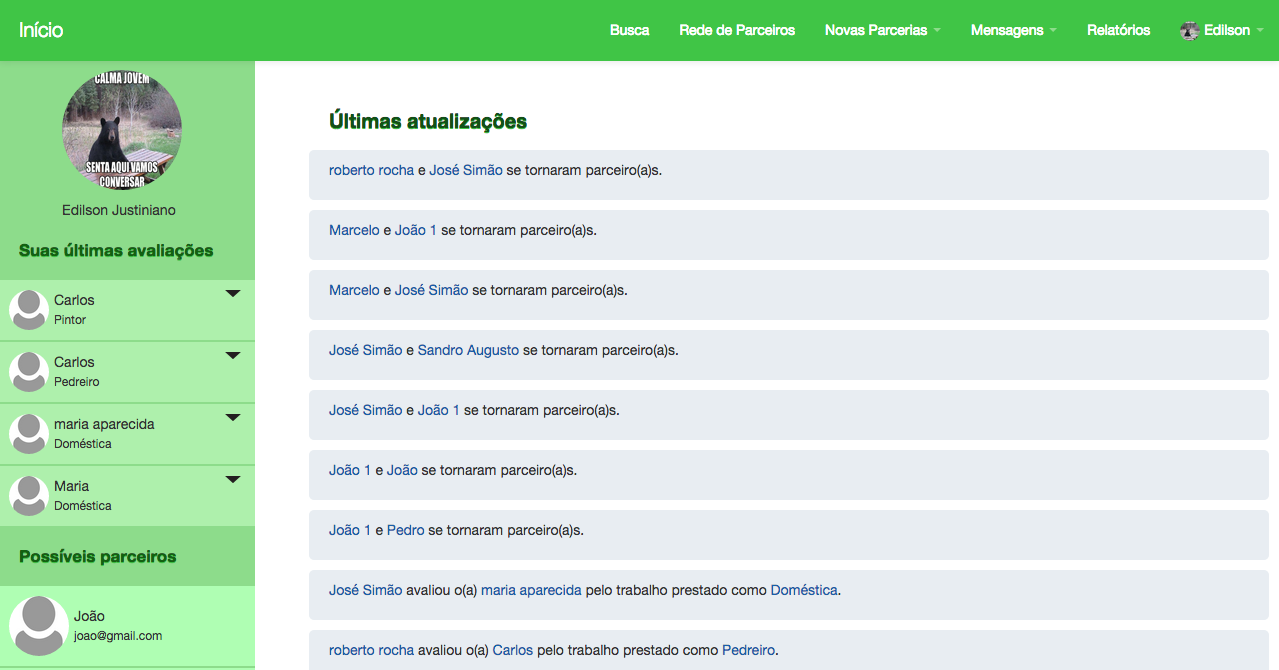
\includegraphics[scale=0.3]{./imagens/home-contratante.png}}
	\caption[Página inicial do usuário contratante.]
	{Página inicial do usuário contratante. \textbf{Fonte:} Elaborado pelos autores.}
	\label{fig:pagina_inicial_contratante}
\end{figure}


\par O caso de uso localizar parceiros foi desenvolvido após a conclusão do caso de uso criar conta. A lógica deste caso de uso consiste em buscar por possíveis parceiros, com base na rede de parceria do contrante. O Código~\ref{list:consulta_possiveis_parceiros} apresenta a consulta realizada no banco de dados a fim de obter essas informações.

\begin{lstlisting} [style=custom_SQL,caption={[\textit{Query} para apresentar possíveis parceiros]{\textit{Query} para apresentar possíveis parceiros. \textbf{Fonte:} Elaborado pelos autores.}}, label=list:consulta_possiveis_parceiros] 	
MATCH (me:Person {email: 'andressa_faria18@hotmal.com'}), (users:Person),
(users)-[:WORKS_IN]->(company)<-[:WORKS_IN]-(me)
WHERE users <> me AND users.typeOfAccount <> 'SERVICE_PROVIDER'
AND NOT((users)-[:PARTNER_OF]->(me)-[:PARTNER_OF]->(users)) 
OPTIONAL MATCH
	pMutualFriends=(me)-[:PARTNER_OF]->(another)-[:PARTNER_OF]->(me),
	(users)-[:PARTNER_OF]->(another)-[:PARTNER_OF]->(users)
RETURN DISTINCT({name: users.name, email: users.email, length: 1, 
photo: users.photo, qtde: count(DISTINCT pMutualFriends)}) as person
ORDER BY person.length, person.qtde DESC
UNION ALL
MATCH (me:Person {email: 'andressa_faria18@hotmal.com'}), (users:Person),
(users)-[:LIVES_IN]->(city)<-[:LIVES_IN]-(me)
WHERE NOT((users)-[:WORKS_IN]->()<-[:WORKS_IN]-(me))
AND users.typeOfAccount <> 'SERVICE_PROVIDER'
AND NOT((users)-[:PARTNER_OF]->(me)-[:PARTNER_OF]->(users))
OPTIONAL MATCH 
	pMutualFriends=(me)-[:PARTNER_OF]->(another)-[:PARTNER_OF]->(me),
	(users)-[:PARTNER_OF]->(another)-[:PARTNER_OF]->(users)
RETURN DISTINCT({name: users.name, email: users.email, length: 2, 
photo: users.photo, qtde: count(DISTINCT pMutualFriends)}) as person
ORDER BY person.length, person.qtde DESC
\end{lstlisting}

\par Essa consulta é dividida em duas sub consultas separadas pela cláusula \texttt{UNION ALL}, a fim de atingir um número maior de possíveis parceiros ao usuário, sendo que a primeira delas está recuperando os dados de pessoas que trabalham na empresa cujo o usuário autenticado no sistema trabalha e não possua o relacionamento de ''parceria'' com ele. A última sub consulta é responsável por obter os dados de pessoas que vivem na cidade cujo o usuário autenticado vive, porém não possuem relacionamento de ''parceria'' e não trabalham na mesma empresa. Ambas as sub consultas levam em consideração os ''parceiros'' em comum entre o contratante autenticado e o possível parceiro. A Figura~\ref{fig:exemplo_funcionamento_possivel_parceiro} exemplifica o funcionamento dessa consulta.

\begin{figure}[h!]
	\centerline{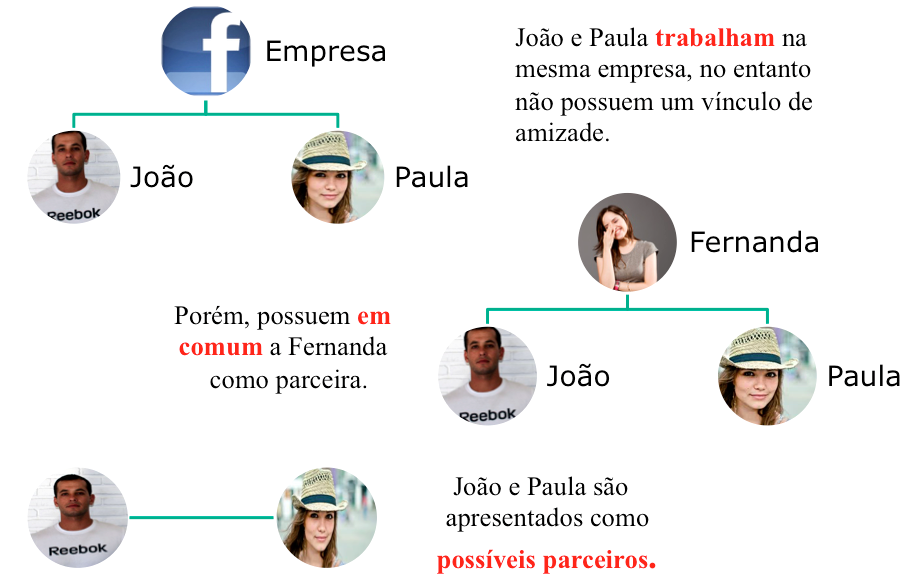
\includegraphics[scale=0.4]{./imagens/exemplo-funcionamento-consulta-possiveis-parceiros.png}}
	\caption[Exemplificação da consulta por possíveis parceiros.]
	{Exemplificação da consulta por possíveis parceiros. \textbf{Fonte:} Elaborado pelos autores.}
	\label{fig:exemplo_funcionamento_possivel_parceiro}
\end{figure}


\par Ainda relacionado ao tipo de conta contratante ou ambos, foi implementado o caso de uso adicionar parceiro, que permite ao usuário convidar um possível parceiro para fazer parte da sua rede.

\par Ao enviar a solicitação de parceria, a aplicação executa uma consulta no banco de dados. Essa consulta é responsável por criar uma aresta entre o nó do usuário autenticado no sistema e o parceiro convidado, conforme apresenta o Código~\ref{list:query_adicionar_parceiro}.

\begin{lstlisting} [style=custom_SQL,caption={[\textit{Query} para enviar solicitação de parceria]{\textit{Query} para enviar solicitação de parceria. \textbf{Fonte:} Elaborado pelos autores.}}, label=list:query_adicionar_parceiro] 	
MATCH (me:Person {email: 'edilsonjustiniano@gmail.com'}),
(partner:Person {email: 'andressa_faria18@hotmail.com'})
CREATE (me)-[:PARTNER_OF {since: 9898723435424281}]->(partner)
RETURN {myName: me.name, myEmail: me.email, partnerName: partner.name, 
partnerEmail: partner.email} as added
\end{lstlisting}

\par Essa consulta é separada em três partes, sendo elas dividas pelas cláusulas \texttt{MATCH}, \texttt{CREATE} e \texttt{RETURN}. A primeira parte dessa consulta irá localizar os vértices cujos \textit{e-mails} sejam semelhantes ao do usuário autenticado no sistema e do parceiro convidado, respectivamente. A segunda parte é responsável por criar a aresta entre os vértices obtidos pela primeira parte da consulta. A terceira e última parte, irá retornar os dados de ambos os usuários, sendo eles, o usuário autenticado no sistema e parceiro recém convidado a fazer parte da rede de parceiros do usuário autenticado.

\par Após a implementação da lógica para adicionar um novo parceiro, houve a necessidade de implementar o serviço de requisições de parcerias, uma vez que não bastava apenas um contratante convidar outro para se tornarem parceiros, mas sim que o contratante convidado aceitasse sua solicitação de parceria, para assim se tornarem parceiros. Visando disponibilizar estas solicitações de forma agradável ao usuário, foi desenvolvida uma funcionalidade para que o usuário pudesse aceitar ou rejeitar a solicitação enviada a ele, essa funcionalidade apresentada em destaque na Figura~\ref{fig:aceitar_rejeitar_solicitacao_parceria}.

\begin{figure}[h!]
	\centerline{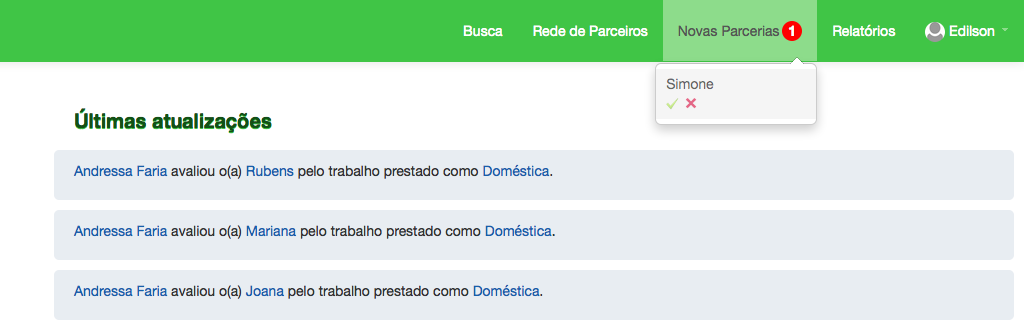
\includegraphics[scale=0.4]{./imagens/aceitar_rejeitar_solicitacao_parceria.png}}
	\caption[Tela para aceitar ou rejeitar solicitação de parceria.]
	{Tela para aceitar ou rejeitar solicitação de parceria. \textbf{Fonte:} Elaborado pelos autores.}
	\label{fig:aceitar_rejeitar_solicitacao_parceria}
\end{figure}

\par A partir dessa funcionalidade, o usuário será capaz de aceitar ou recusar a solicitação apenas com um \textit{click}. Caso o usuário aceite a solicitação, o sistema irá realizar os procedimentos necessários e irá executar a mesma consulta apresentada no Código~\ref{list:query_adicionar_parceiro}, porém com os \textit{e-mails} invertidos. Essa consulta será reutilizada, pois, para que dois usuários se tornem parceiros é necessário que ambos possuam uma aresta do tipo \texttt{PARTNER OF} apontando um ao outro.

\par Se o usuário rejeitar a solicitação, o sistema realizará os procedimentos necessários e executará a consulta apresentada no Código~\ref{list:query_remover_parceiro} a fim de excluir a aresta criada anteriormente pela solicitação de parceria.

\begin{lstlisting} [style=custom_SQL,caption={[\textit{Query} para remover solicitação de parceria]{\textit{Query} para remover solicitação de parceria. \textbf{Fonte:} Elaborado pelos autores.}}, label=list:query_remover_parceiro] 	
MATCH (me:Person {email: 'andressa_faria18@hotmail.com'}),
(partner:Person {email: 'edilsonjustiniano@gmail.com'}),
(partner)-[rel:PARTNER_OF]->(me)
DELETE rel
RETURN {myName: me.name, myEmail: me.email, 
partnerName: partner.name, partnerEmail: partner.email} as deleted;
\end{lstlisting}

\par Essa consulta, a exemplo da anterior, é separada em três partes, sendo elas dividas pelas cláusulas \texttt{MATCH}, \texttt{DELETE} e \texttt{RETURN}. A primeira parte dessa consulta irá localizar os vértices cujos \textit{e-mails} sejam semelhantes ao do usuário autenticado no sistema e do parceiro convidado, respectivamente, e que possuam uma aresta do tipo \texttt{PARTNER OF} os conectando, porém, essa aresta se inicia no vértice relacionado ao parceiro convidado e o final seja vértice relacionado ao usuário autenticado. A segunda parte consiste apenas na exclusão da aresta obtida na primeira parte da consulta. A terceira e última parte, irá retornar os dados de ambos os usuários, sendo eles, o usuário autenticado no sistema e parceiro cujo, convite para se tornar parceiro foi rejeitado pelo usuário autenticado no sistema.

\par Após realizada a implementação do caso de uso adicionar parceiro, houve a necessidade de desenvolver a busca por todos os usuários que possuíam o tipo de conta contratante ou ambos e que possuíam um relacionamento de parceria com o usuário autenticado no sistema, além da funcionalidade de localizar novos parceiros, baseando-se na localização da empresa na qual o usuário trabalha e na cidade onde ele vive, sempre ordenando os resultados por meio da quantidade de parceiros em comum. O Código~\ref{list:consulta_novos_parceiros} apresenta a \textit{query} utilizada para realizar esta busca.

\begin{lstlisting} [style=custom_SQL,caption={[\textit{Query} para apresentar novos parceiros]{\textit{Query} para apresentar novos parceiros. \textbf{Fonte:} Elaborado pelos autores.}}, label=list:consulta_novos_parceiros] 	
MATCH (me:Person {email: 'andressa_faria18@hotmail.com'}), (users:Person),
(users)-[:WORKS_IN]->(company)<-[:WORKS_IN]-(me)
WHERE users.name =~ 'Edil.*'
AND users.typeOfAccount <> 'SERVICE_PROVIDER'
AND users <> me AND NOT((users)-[:PARTNER_OF]->(me)-[:PARTNER_OF]->(users))  
OPTIONAL MATCH 
	pMutualFriends=(me)-[:PARTNER_OF]->(another)-[:PARTNER_OF]->(me), 
	(users)-[:PARTNER_OF]->(another)-[:PARTNER_OF]->(users) 
RETURN DISTINCT({name: users.name, email: users.email, length: 1, 
photo: users.photo, mutualFriends: count(DISTINCT pMutualFriends)}) 
as partner ORDER BY partner.length, partner.mutualFriends DESC 
UNION ALL 
MATCH (me:Person {email: 'andressa_faria18@hotmail.com'}), (users:Person),
(users)-[:LIVES_IN]-(city)<-[:LIVES_IN]-(me)
WHERE users.name =~ 'Edil.*'
AND users.typeOfAccount <> 'SERVICE_PROVIDER' 
AND NOT((users)-[:WORKS_IN]->()<-[:WORKS_IN]-(me)) 
AND NOT((users)-[:PARTNER_OF]->(me)-[:PARTNER_OF]->(users)) 
OPTIONAL MATCH 
	pMutualFriends=(me)-[:PARTNER_OF]->(another)-[:PARTNER_OF]->(me), 
	(users)-[:PARTNER_OF]->(another)-[:PARTNER_OF]->(users) 
RETURN DISTINCT({name: users.name, email: users.email, length: 2, 
photo: users.photo, mutualFriends: count(DISTINCT pMutualFriends)})
as partner ORDER BY partner.length, partner.mutualFriends DESC
\end{lstlisting}

\par Essa consulta é muito parecida com a apresentada no Código~\ref{list:consulta_possiveis_parceiros}, porém há uma diferença, neste caso é levado em consideração o nome informado pelo usuário como critério de busca.
 

\par O caso de uso ''Gerenciar serviços'' foi implementado em sequência, abrangendo as principais funcionalidades de gerenciamento: cadastrar e adicionar um novo serviço ao usuário, cujo tipo de conta é provedor de serviços, listar os serviços atribuídos a ele, e remover serviços quando necessário. Visando melhorar a usabilidade, foi implementado um mecanismo de busca, que permitiu filtrar os resultados por meio de um campo que possui a função  auto completar, evitando assim, possíveis erros e diminuindo o tempo gasto pelo usuário para adicionar o serviço. A função realiza a busca em uma lista de serviços anteriormente cadastrados, no entanto, caso não haja o serviço solicitado, o usuário tem a liberdade de cadastrá-lo e atribuí-lo a si mesmo. A Figura~\ref{fig:adicionar_servicos} apresenta essa funcionalidade.

\newpage
\begin{figure}[h!]
	\centerline{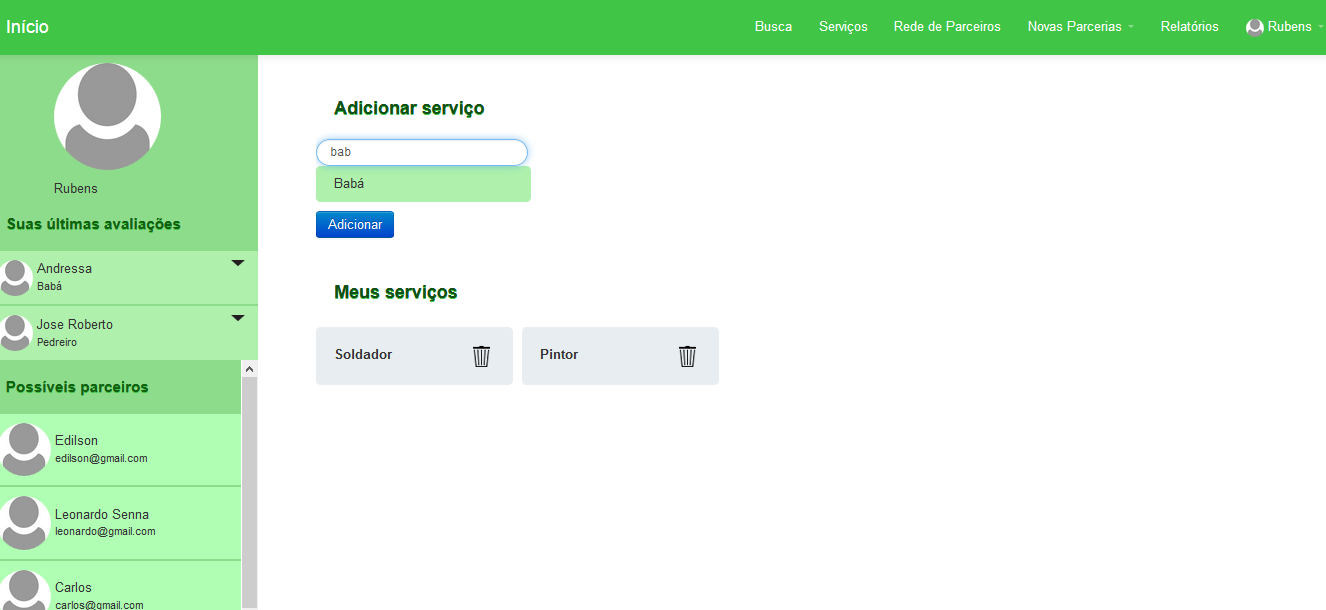
\includegraphics[scale=0.3]{./imagens/adcionar-servico.png}}
	\caption[Página para adicionar serviços.]
	{Página para adicionar serviços. \textbf{Fonte:} Elaborado pelos autores.}
	\label{fig:adicionar_servicos}
\end{figure}


\par A partir deste ponto, foi possível iniciar o desenvolvimento do caso de uso "localizar mão de obra", uma vez que, este caso de uso dependia diretamente das implementações das funcionalidades adicionar parceiros para os usuários contratantes e adicionar serviços aos provedores de serviço. Para facilitar a localização e deixar o \textit{software} mais usual, esta busca se baseia inicialmente no serviço buscado pelo usuário, sendo posteriormente modificada para também levar em consideração a funcionalidade, avaliar serviço que foi implementada paralelamente. A avaliação de serviço permite ao contratante dar uma nota ao serviço que foi prestado a ele. Com estas informações foi possível desenvolver uma busca que levaria em consideração, além destas informações, a rede de parceiros do usuário contratante, a fim de lhe apresentar as melhores opções possíveis. O Código~\ref{list:consulta_busca} apresenta a \textit{query} utilizada para realizar esta busca.


\begin{lstlisting} [style=custom_SQL,caption={[\textit{Query} para localização de mão de obra]{\textit{Query} para localização de mão de obra. \textbf{Fonte:} Elaborado pelos autores.}}, label=list:consulta_busca] 	
MATCH (me:Person {email: 'edilsonjustiniano@gmail.com'}), (sp:Person), 
(service:Service), (executed:Execute), (partners:Person), 
(partners)-[:PARTNER_OF]->(me)-[:PARTNER_OF]->(partners),
(sp)-[:PROVIDE]->(service), (service)-[:EXECUTE]->(executed),
(sp)-[:EXECUTE]->(executed)
WHERE sp.typeOfAccount <> 'CONTRACTOR' 
AND partners.typeOfAccount <> 'SERVICE_PROVIDER'
AND UPPER(service.name) = UPPER('Domestica')
AND (executed)-[:TO]->(partners) AND me <> sp
RETURN DISTINCT({serviceProviderName: sp.name, 
serviceProviderEmail: sp.email, service: service.name,
total: count(executed), media: avg(executed.note), order: 1}) as sp 
ORDER BY sp.order, sp.media DESC
UNION ALL
MATCH (me:Person {email: 'edilsonjustiniano@gmail.com'}), (sp:Person),
(service:Service {name: 'Domestica'}), (executed:Execute),
(partners:Person), (partners)-[:WORKS_IN]->(company)<-[:WORKS_IN]-(me),
(sp)-[:PROVIDE]->(service), (service)-[:EXECUTE]->(executed), 
(sp)-[:EXECUTE]->(executed), (executed)-[:TO]->(partners)
WHERE sp.typeOfAccount <> 'CONTRACTOR' 
AND partners.typeOfAccount <> 'SERVICE_PROVIDER'
AND NOT((partners)-[:PARTNER_OF]->(me)-[:PARTNER_OF]->(partners))
AND me <> sp
RETURN DISTINCT({serviceProviderName: sp.name, 
serviceProviderEmail: sp.email, service: service.name, 
total: count(executed), media: avg(executed.note), order: 2}) as sp 
ORDER BY sp.order, sp.media DESC
UNION ALL
MATCH (me:Person {email: 'edilsonjustiniano@gmail.com'}), (sp:Person),
(service:Service {name: 'Domestica'}), (executed:Execute), 
(partners:Person), (partners)-[:LIVES_IN]->(city)<-[:LIVES_IN]-(me),
(sp)-[:PROVIDE]->(service), (service)-[:EXECUTE]->(executed), 
(sp)-[:EXECUTE]->(executed), (executed)-[:TO]->(partners)
WHERE sp.typeOfAccount <> 'CONTRACTOR' 
AND partners.typeOfAccount <> 'SERVICE_PROVIDER'
AND NOT((partners)-[:PARTNER_OF]->(me)-[:PARTNER_OF]->(partners))
AND NOT((partners)-[:WORKS_IN]->()<-[:WORKS_IN]-(me))
AND me <> sp
RETURN DISTINCT({serviceProviderName: sp.name, 
serviceProviderEmail: sp.email, service: service.name, 
total: count(executed), media: avg(executed.note), order: 3}) as sp 
ORDER BY sp.order, sp.media DESC 
UNION ALL
MATCH (me:Person {email: 'edilsonjustiniano@gmail.com'}), (sp:Person),
(service:Service {name: 'Domestica'}), (partners:Person),
(partners)-[:LIVES_IN]->(city)<-[:LIVES_IN]-(me), 
(sp)-[:PROVIDE]->(service)
WHERE sp.typeOfAccount <> 'CONTRACTOR' 
AND partners.typeOfAccount <> 'SERVICE_PROVIDER'
AND NOT((partners)-[:PARTNER_OF]->(me)-[:PARTNER_OF]->(partners))
AND NOT((partners)-[:WORKS_IN]->()<-[:WORKS_IN]-(me))
AND me <> sp
RETURN DISTINCT({serviceProviderName: sp.name, 
serviceProviderEmail: sp.email, service: service.name, total: 0,
media: 0, order: 4}) as sp ORDER BY sp.order, sp.media DESC;
\end{lstlisting}

Essa consulta é dividida em quatro sub consultas, separadas pela cláusula \texttt{UNION ALL}, a fim de atingir um número maior de possibilidades de prestadores de serviços. Visando facilitar o entendimento, suas partes são apresentadas isoladamente a seguir.

A primeira delas está recuperando os dados de pessoas que proveram o serviço de doméstica para usuários que possuem o relacionamento de parceria com o usuário autenticado no sistema, nesse caso o \textit{e-mail} dele é \texttt{edilsonjustiniano@gmail.com}. Portanto, nessa primeira parte da consulta serão retornadas as avaliações realizadas pelos parceiros do usuário autenticado no sistema voltadas às pessoas que proveem o serviço de doméstica. Essa sub consulta é demonstrada no trecho de Código~\ref{list:consulta_busca_parte1}.

\begin{lstlisting} [style=custom_SQL,caption={[Primeira \textit{sub query} para localização de mão de obra.]{Primeira \textit{sub query} para localização de mão de obra. \textbf{Fonte:} Elaborado pelos autores.}}, label=list:consulta_busca_parte1] 	
MATCH (me:Person {email: 'edilsonjustiniano@gmail.com'}), (sp:Person), 
(service:Service), (executed:Execute), (partners:Person), 
(partners)-[:PARTNER_OF]->(me)-[:PARTNER_OF]->(partners),
(sp)-[:PROVIDE]->(service), (service)-[:EXECUTE]->(executed),
(sp)-[:EXECUTE]->(executed)
WHERE sp.typeOfAccount <> 'CONTRACTOR' 
AND partners.typeOfAccount <> 'SERVICE_PROVIDER'
AND UPPER(service.name) = UPPER('Domestica')
AND (executed)-[:TO]->(partners) AND me <> sp
RETURN DISTINCT({serviceProviderName: sp.name, 
serviceProviderEmail: sp.email, service: service.name,
total: count(executed), media: avg(executed.note), order: 1}) as sp 
ORDER BY sp.order, sp.media DESC
\end{lstlisting}

A segunda sub consulta irá obter os dados de pessoas que proveram o mesmo serviço da sub consulta anterior para usuários que trabalhem na mesma empresa, mas que não possuem o relacionamento de parceria com o usuário autenticado no sistema. Portanto, nessa segunda parte da consulta serão retornados as avaliações realizadas por pessoas que não são parceiras do usuário autenticado no sistema, mas que trabalham na mesma empresa. Essa sub consulta é demonstrada no trecho de Código~\ref{list:consulta_busca_parte2}.

\begin{lstlisting} [style=custom_SQL,caption={[Segunda \textit{sub query} para localização de mão de obra.]{Segunda \textit{sub query} para localização de mão de obra. \textbf{Fonte:} Elaborado pelos autores.}}, label=list:consulta_busca_parte2] 	
MATCH (me:Person {email: 'edilsonjustiniano@gmail.com'}), (sp:Person),
(service:Service {name: 'Domestica'}), (executed:Execute),
(partners:Person), (partners)-[:WORKS_IN]->(company)<-[:WORKS_IN]-(me),
(sp)-[:PROVIDE]->(service), (service)-[:EXECUTE]->(executed), 
(sp)-[:EXECUTE]->(executed), (executed)-[:TO]->(partners)
WHERE sp.typeOfAccount <> 'CONTRACTOR' 
AND partners.typeOfAccount <> 'SERVICE_PROVIDER'
AND NOT((partners)-[:PARTNER_OF]->(me)-[:PARTNER_OF]->(partners))
AND me <> sp
RETURN DISTINCT({serviceProviderName: sp.name, 
serviceProviderEmail: sp.email, service: service.name, 
total: count(executed), media: avg(executed.note), order: 2}) as sp 
ORDER BY sp.order, sp.media DESC
\end{lstlisting}

Já a terceira sub consulta irá obter os dados de pessoas que proveram o mesmo serviço das sub consultas anteriores para usuários que vivem na mesma cidade que o usuário autenticado no sistema, mas que não trabalhem na mesma empresa que ele e não possuam o relacionamento de parceria com ele. Portanto, nessa terceira parte da consulta serão retornadas as avaliações realizadas por pessoas que não são parceiras do usuário autenticado no sistema, que não trabalhem na mesma empresa dele, mas que vivam na mesma cidade. Essa sub consulta é demonstrada no trecho de Código~\ref{list:consulta_busca_parte3}.

\begin{lstlisting} [style=custom_SQL,caption={[Terceira \textit{sub query} para localização de mão de obra.]{Terceira \textit{sub query} para localização de mão de obra. \textbf{Fonte:} Elaborado pelos autores.}}, label=list:consulta_busca_parte3] 	
MATCH (me:Person {email: 'edilsonjustiniano@gmail.com'}), (sp:Person),
(service:Service {name: 'Domestica'}), (executed:Execute), 
(partners:Person), (partners)-[:LIVES_IN]->(city)<-[:LIVES_IN]-(me),
(sp)-[:PROVIDE]->(service), (service)-[:EXECUTE]->(executed), 
(sp)-[:EXECUTE]->(executed), (executed)-[:TO]->(partners)
WHERE sp.typeOfAccount <> 'CONTRACTOR' 
AND partners.typeOfAccount <> 'SERVICE_PROVIDER'
AND NOT((partners)-[:PARTNER_OF]->(me)-[:PARTNER_OF]->(partners))
AND NOT((partners)-[:WORKS_IN]->()<-[:WORKS_IN]-(me))
AND me <> sp
RETURN DISTINCT({serviceProviderName: sp.name, 
serviceProviderEmail: sp.email, service: service.name, 
total: count(executed), media: avg(executed.note), order: 3}) as sp 
ORDER BY sp.order, sp.media DESC 
\end{lstlisting}

Já a quarta e última sub consulta foi inserida a fim de abranger a busca e possibilitar que novos prestadores de serviços sejam avaliados pelos contratantes. Ela irá obter os dados de pessoas que ainda não foram avaliadas por nenhum parceiro, ou por pessoas que vivam na mesma cidade ou trabalhem na mesma empresa do usuário autenticado no sistema, o que permitiu aos usuários que acabaram de criar sua conta e não obtiveram a oportunidade de serem avaliados que fossem apresentados como opções para o serviço. Essa sub consulta é demonstrada no trecho de Código~\ref{list:consulta_busca_parte4}.

\begin{lstlisting} [style=custom_SQL,caption={[Quarta \textit{sub query} para localização de mão de obra.]{Quarta \textit{sub query} para localização de mão de obra. \textbf{Fonte:} Elaborado pelos autores.}}, label=list:consulta_busca_parte4] 	
MATCH (me:Person {email: 'edilsonjustiniano@gmail.com'}), (sp:Person),
(service:Service {name: 'Domestica'}), (partners:Person),
(partners)-[:LIVES_IN]->(city)<-[:LIVES_IN]-(me), 
(sp)-[:PROVIDE]->(service)
WHERE sp.typeOfAccount <> 'CONTRACTOR' 
AND partners.typeOfAccount <> 'SERVICE_PROVIDER'
AND NOT((partners)-[:PARTNER_OF]->(me)-[:PARTNER_OF]->(partners))
AND NOT((partners)-[:WORKS_IN]->()<-[:WORKS_IN]-(me))
AND me <> sp
RETURN DISTINCT({serviceProviderName: sp.name, 
serviceProviderEmail: sp.email, service: service.name, total: 0,
media: 0, order: 4}) as sp ORDER BY sp.order, sp.media DESC
\end{lstlisting}

\par A Figura~\ref{fig:explificar_consulta_busca_mao_de_obra} exemplifica todo o funcionamento da consulta de forma detalhada, facilitando a compreensão desta, que é, a maior e mais complexa consulta deste trabalho.

\begin{figure}[h!]
	\centerline{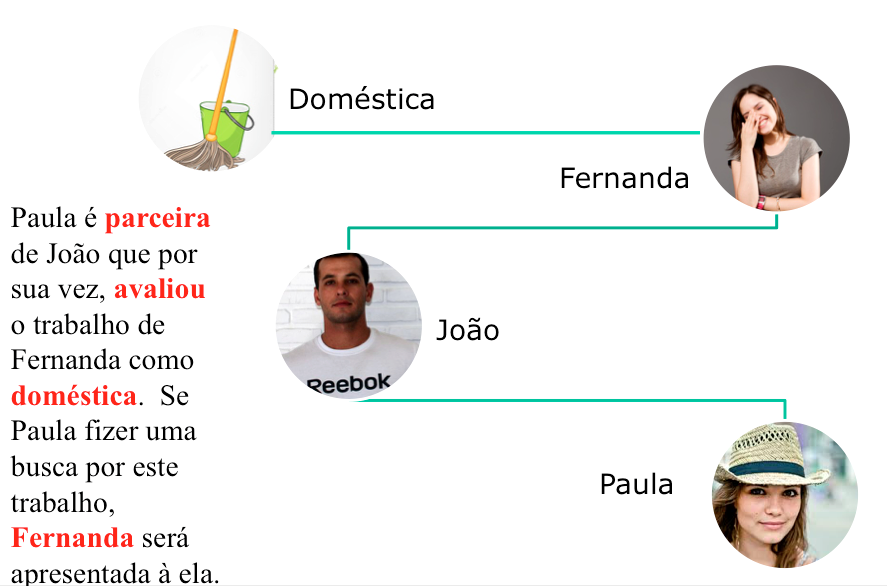
\includegraphics[scale=0.4]{./imagens/exemplo-funcionamento-consulta-buscar-mao-de-obra.png}}
	\caption[Exemplificação da consulta por mão de obra.]
	{Exemplificação da consulta por mão de obra. \textbf{Fonte:} Elaborado pelos autores.}
	\label{fig:explificar_consulta_busca_mao_de_obra}
\end{figure}


\par Para auxiliar na tomada de decisão do usuário contratante, foi implementada uma funcionalidade que realiza o cálculo da média de avaliação de um serviço prestado por um profissional temporário, tendo como base as avaliações já realizadas pela rede de parceiros do usuário autenticado, da empresa onde ele trabalha e da cidade onde vive, oferecendo assim uma forma simples de obter acesso a qualidade do serviço prestado como demonstra a Figura~\ref{fig:taxa_avaliacao}.

\begin{figure}[h!]
	\centerline{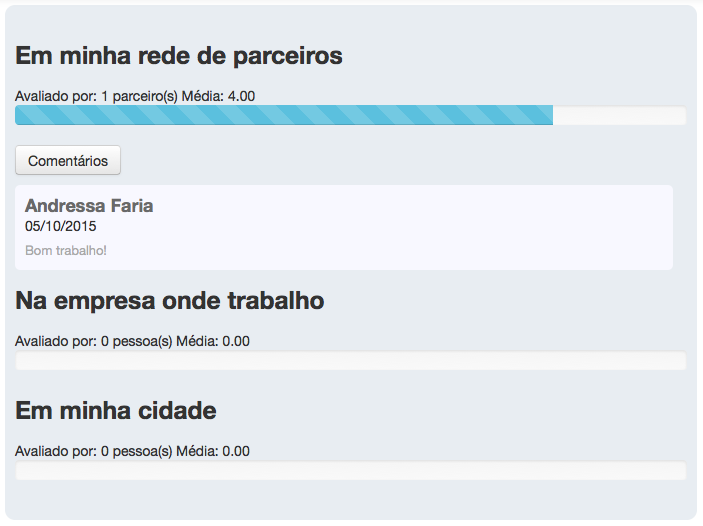
\includegraphics[scale=0.45]{./imagens/taxa-avaliacao.png}}
	\caption[Tela contendo a taxa de avaliação do serviço prestado.]
	{Tela contendo a taxa de avaliação do serviço prestado. \textbf{Fonte:} Elaborado pelos autores.}
	\label{fig:taxa_avaliacao}
\end{figure}

\par Após realizada todas as implementações já descritas, houve a preocupação de desenvolver uma interface, que além de amigável fosse prática ao usuário, desta forma, foi disponibilizada algumas informações relevantes, que auxiliam o usuário a compreender o que está ocorrendo em sua rede de parceria. Como exemplo é possível citar a lista de parceiros em comum entre o usuário autenticado no sistema e um determinado contratante por meio da página de perfil dele.

\par A fim de agregar mais funcionalidades para o usuário provedor de serviços, foi criado na página inicial do \textit{software} uma funcionalidade que visa apresentar algumas dicas interessantes que contribuem com a sua imagem perante ao \textit{software}, levando-o assim a obter uma quantidade maior de oportunidades de trabalho como mostra a Figura~\ref{fig:dicas_randomicas}.

\newpage
\begin{figure}[h!]
	\centerline{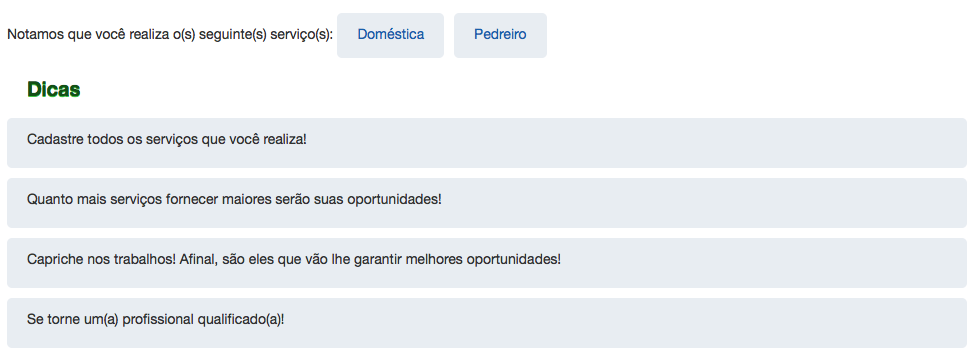
\includegraphics[scale=0.4]{./imagens/dicas-randomicas.png}}
	\caption[Tela de dicas para provedores de serviços.]
	{Tela de dicas para provedores de serviços. \textbf{Fonte:} Elaborado pelos autores.}
	\label{fig:dicas_randomicas}
\end{figure}

\par Para finalizar o desenvolvimento foram desenvolvidos gráficos que apresentem ao usuário informações a respeito da qualidade do serviço prestado pelo provedor de serviços, comparando-os com os demais prestadores. Esses gráficos foram gerados usando a biblioteca chamada \textit{Charts}, disponibilizada no \textit{link} https://developers.google.com/chart. Para utilizá-la, é preciso realizar o \textit{download} e, após concluído, incluir o arquivo chamado \texttt{Charts.js} na página, cujo o gráfico será apresentado, conforme demonstra o Código~\ref{list:codigo_insercao_charts}.

\begin{lstlisting} [style=custom_HTML,caption={[Inserção da biblioteca \textit{charts} na página inicial.]{Inserção da biblioteca \textit{charts} na página inicial. \textbf{Fonte:} Elaborado pelos autores.}}, label=list:codigo_insercao_charts] 	
<script type="text/javascript" src="js/charts/Chart.js"></script>
\end{lstlisting}

\par Para gerar um gráfico, segundo a sua própria documentação, e conforme utilizado neste trabalho, deve-se incluir um elemento \texttt{div} contendo um \texttt{canvas} com um \texttt{id} único, a fim de facilitar o acesso a ele, por meio do código Javascript, que irá manipular os dados apresentados neste gráfico. Essa inclusão do elemento é apresentado no Código~\ref{list:codigo_incluir_canvas_charts}.

\begin{lstlisting} [style=custom_HTML,caption={[Inclusão do elemento necessário para geração do gráfico.]{Inclusão do elemento necessário para geração do gráfico. \textbf{Fonte:} Elaborado pelos autores.}}, label=list:codigo_incluir_canvas_charts] 	
<div>
	<canvas id="canvas" height="450" width="600"></canvas>
</div>
\end{lstlisting}

\par Para manipular as informações do gráfico, tais como dados, cores, entre outras, é necessário criar um objeto em Javascript que contenha todos os atributos necessários para gerá-lo corretamente. Este objeto é apresentado no Código~\ref{list:codigo_objeto_grafico}.

\begin{lstlisting} [style=custom_HTML,caption={[Objeto contendo os atributos de configuração do gráfico.]{Objeto contendo os atributos de configuração do gráfico. \textbf{Fonte:} Elaborado pelos autores.}}, label=list:codigo_objeto_grafico] 	
$scope.lineChartData = {
	labels : ["5 ultimas","10 ultimas","15 ultimas","20 ultimas"],
	datasets : [{
		label: "Minhas avaliacoes como " + $scope.selectedService,
		fillColor : "rgba(166,246,166,0.2)",
		strokeColor : "rgba(61,213,61,1)",
		pointColor : "rgba(61,213,61,1)",
		pointStrokeColor : "#fff",
		pointHighlightFill : "#fff",
		pointHighlightStroke : "rgba(41,157,41,1)",
		data : [
			//filled by lastEvaluateOfServiceProvider
		]   
	}, {
		label: "As avaliacoes de " + $scope.selectedService + " em minha cidade",
		fillColor : "rgba(98,168,248,0.2)",
		strokeColor : "rgba(25,123,235,1)",
		pointColor : "rgba(25,123,235,1)",
		pointStrokeColor : "#fff",
		pointHighlightFill : "#fff",
		pointHighlightStroke : "rgba(33,97,170,1)",
		data : [
			//filled by lastEvaluateOfServiceInNetwork
		]
	}]
};
\end{lstlisting}

\par Após realizados os passos anteriormente descritos, para finalizar a geração do gráfico, foi necessário criar uma nova instância da classe \texttt{Chart}, informando o modelo do gráfico a ser utilizado, nesse caso, o modelo de linhas, a fim de facilitar a comparação entre as avaliações, juntamente com o objeto contendo todas as informações do gráfico, conforme apresentado na linha 3 do Código~\ref{list:codigo_criar_grafico_charts} que demonstra a criação dessa nova instância.

\begin{lstlisting} [style=custom_HTML,caption={[Criação de nova instância para gráficos de linha.]{Criação de nova instância para gráficos de linha. \textbf{Fonte:} Elaborado pelos autores.}}, label=list:codigo_criar_grafico_charts] 	
$scope.loadGraph = function(){
	var ctx = document.getElementById("canvas").getContext("2d");
	window.myLine = new Chart(ctx).Line($scope.lineChartData, {
		responsive: true
	});
};
\end{lstlisting}

\par Essa biblioteca foi selecionada, pois, ela é facilmente integrada com o \textit{framework} Angular JS, facilitando a sua utilização neste trabalho. 

\par O primeiro gráfico foi disponibilizado na página de perfil do prestador de serviços, estando visível ao contratante assim que ele efetue a busca por uma mão de obra. Este gráfico apresenta a média avaliativa dos trabalhos prestados pelo provedor selecionado em uma determinada função. O sistema toma como base as vinte últimas avaliações recebidas, independente do período em que elas foram feitas. Desta forma, um provedor de serviços que trabalha a muito tempo em um mesmo local não será prejudicado, pois terá registrada as avaliações que recebeu neste tempo, mesmo que elas não sejam atuais. O gráfico que representa esta funcionalidade é apresentado na Figura \ref{fig:grafico_pagina_perfil}.

\begin{figure}[h!]
	\centerline{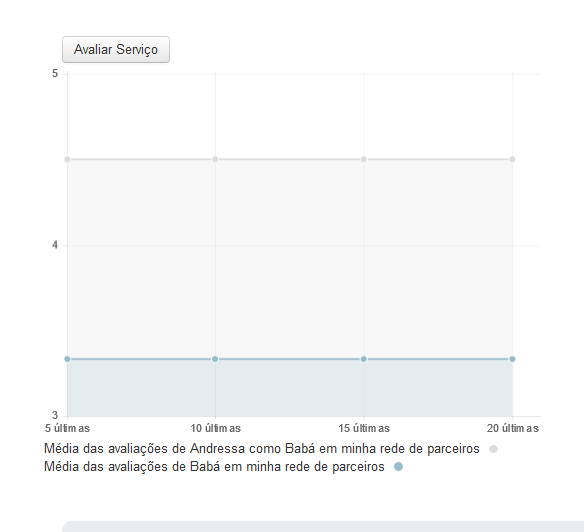
\includegraphics[scale=0.65]{./imagens/grafico-pagina-perfil.png}}
	\caption[Gráfico de avaliação do serviço na página de perfil do provedor.]
	{Gráfico de avaliação do serviço na página de perfil do provedor. \textbf{Fonte:} Elaborado pelos autores.}
	\label{fig:grafico_pagina_perfil}
\end{figure}

\par O segundo gráfico foi disponibilizado visando possibilitar ao prestador de serviços ter um \textit{feedback} dos trabalhos realizados por ele. Este gráfico é apresentado em sua página inicial e trás informações referente a sua média avaliativa. A média é gerada com base nas últimas vinte avaliações recebidas, seguindo o mesmo padrão do gráfico disponibilizado na página de perfil. Para que o provedor tenha uma base da qualidade do serviço prestado, o gráfico apresenta um comparatiParavo da média recebida por ele e a média geral de prestadores de serviço que desempenham o mesmo trabalho em sua cidade. O gráfico que representa esta funcionalidade é apresentado na Figura \ref{fig:grafico_pagina_inicial}.

\newpage
\begin{figure}[h!]
	\centerline{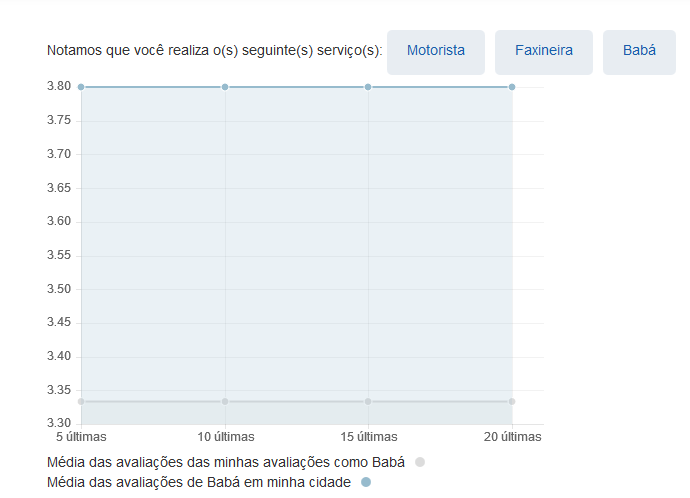
\includegraphics[scale=0.65]{./imagens/grafico-pagina-inicial.png}}
	\caption[Gráfico de avaliação do serviço na página inicial do provedor.]
	{Gráfico de avaliação do serviço na página inicial do provedor. \textbf{Fonte:} Elaborado pelos autores.}
	\label{fig:grafico_pagina_inicial}
\end{figure}

\par Seguindo todos os procedimentos descritos nessa seção obteve-se como resultado a aplicação proposta por este trabalho.